\documentclass{article}
\usepackage{graphicx} 
\usepackage{amsmath}
\usepackage{tikz}
\usetikzlibrary{positioning}

\title{Project-2}
\author{Polisetty Tharun Sai}
\date{2023CSB1144}

\begin{document}

\maketitle

\section*{Question1: Choose the top leader by running a random walk on the graph with teleportation.}
\subsection*{Answer:}
\paragraph{First i read the Impression network.xlsx provided by using pandas library.\\ Then storing the column of Email addresses in a variable will provide us the nodes in out network.\\ But when we observe the given instances in the email addresses column are in form of email id , So since we have an unique node value i have converted an email id to an unique id based on the following conversion. 
   $$ yyyyabcijkl@iitrpr.ac.in =  yyyyijkl $$}
\paragraph{Then , i stored each row as a sublist in a column ,  which means the neighbours of the node in email address are present in the respective index of the rows list.\\And again here problem arised because the provided xl sheet has name also with the entry number which I will remove for making further calculations easier as all these neighbours also should be same as how nodes are present. $$name yyyyABCijkl = yyyyijikl$$ }
\paragraph{Now only thing to do is to apply the page rank finding through processing a random walk.}
\subsubsection*{Random Walk:}
\paragraph{1)Choose a Random Node.\\2)Increase points of for each node that we arrive.\\3)Now if the node has a neighbour then we choose a random neighbour of them , and if there are no neighbours for that node then we teleport from that node and choose a random node in the graph again.\\4)But now consider a situation where two nodes have links in between them but there are no outlinks for them to the rest of the network. Then if our walk approached one of the above two nodes the walk would follow only those two nodes in a loop and the rank of them will become the highest. So we must have a probability for teleporting although a node has neighbours so we are fixing a 0.15 probability for a teleportation to occur irrespective of there are neighbours or not.}
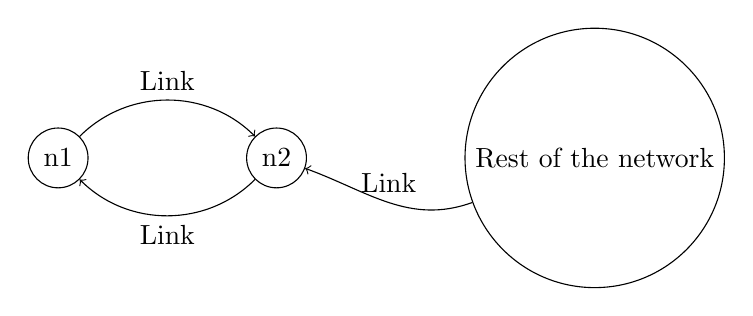
\begin{tikzpicture}[node distance=2cm]
    \node[draw,circle] (n1) {n1};
    \node[draw,circle,right=of n1] (n2) {n2};
    \node[draw,circle,right=of n2] (rest) {Rest of the network};
    \draw[->] (n1) to[out=45,in=135] node[above] {Link} (n2);
    \draw[->] (n2) to[out=225,in=315] node[below] {Link} (n1);
    \draw[->] (rest) to[out=200,in=340] node[above] {Link} (n2);
\end{tikzpicture}
\paragraph{5)Now we will start our random walk and find out the page rank by limiting our steps by some large number such as 1L or 10L.}
\newpage
\section*{Question2: Recommend missing links using the matrix method explained in the class.}
\subsection*{Missing edges Matrix Method:}
\paragraph{What is a Missing link? A missing link that edge which is not existing in real time but if those two nodes if they were to meet each each other then there would be an edge between them. That is expecting the relation between two nodes if there were a meet between them.}
\subsection*{Matrix Method:}
\paragraph{This method is used for expecting missing elements of a matrix when we have data of some entries in it. Here we are considering a row as a linear combination of the known rows and on calculating the coefficients of that linear combination we will expect this linear combination is followed with all the unknown entries also.\\Since here we are expecting missing edges it means nothing but the missing 1's in the adjacency matrix in place of existing 0's.\\So if we have a[i][j] of the adjacency matrix to be 0 ,then we take the linear combination of the rest of the rows and rest of the columns and expect our a[i][j] with our process explained below.}
\paragraph{Consider a matrix A which is the adjacency matrix with the i-th row and j-th column removed, denoted as $A_{ij}$.\\ Also, let's define a row matrix B, denoted as $B_i$, which is the i-th row of the adjacency matrix with the j-th element removed.\\ We now have to express the row matrix $B_i$ as a linear combination of the rows of matrix $A_{ij}$, denoted as $$c_1A_1 + c_2A_2 + \ldots + c_nA_n$$, where $A_k$ represents the k-th row of matrix $A_{ij}$ and $c_k$ represents the coefficients of the linear combination.\\Now let us name the column matrix $X_{ij}$ which is a column matrix whose entries are the above ci's.$$A_{i,j}X_{i,j}=B_{i}$$\\Now for expecting whether there will be a 1 or 0 at a[i][j]. \\ So we define a column matrix C , denoted as $C_j$. Now we will make a dot product which is nothing but writing our unknown entry a[i][j]. And if this dot product is greater than 0 then we expect there must be an edge present. But if its not the case then that edge remained unconnected.}


\section*{Question3: Propose a brand new problem based on this dataset and provide a solution for the same. Be as creative as possible.}
\subsection*{Question I thought of : Check whether the given Impressions Network data is following Ideal distribution? and if it's not ,then give the IDs of those students who are violating ideal nature.}
\paragraph{Firstly, why choose this question. Because whenever one have a data it is very important to check How reliable that data is i,e., How normal this data is to believe so that we are confident to rely on it. And this is done nowadays in many ways for example:\\i)Histograms and frequency Distributions. \\ii)Box Plots. \\iii)Q-Q plot. \\iv)P-P plot.\\ Among these above one can use any of the method but here I am using the Histograms method which is considered as one of the standard statistical way of realising a data. \\ \\ \underline{Histograms and Frequency Distributions }: A histogram is an estimate of the probability distribution of a variable. If the graph is approximately bell-shaped and symmetric about the mean ,it shows normal behaviour.}
\paragraph{\\}
\begin{figure}[h]
  \centering
  \includegraphics[width=0.7\textwidth]{image.png}
  \caption{Bell Curve or Normal Distribution}
\end{figure}

\paragraph{{\Large
\[ y = \dfrac{1}{\sigma\sqrt{2\pi}} e^{-\frac{(x-\mu)^{2}}{2\sigma^{2}}} \]
}\\ $\mu = Mean \\ \sigma = Standard Deviation $}
 \begin{figure}
    \centering
    \includegraphics[width=0.6
    \linewidth]{Discrete_Math.png}
    \caption{The Frequency distribution Observed }
    \label{fig:enter-label}
\end{figure} 
\paragraph{In our situation I took the frequency parameter as:\\Since the number of out-links from a graph in a small network like our case might not be very normally distributed as if we observe there are more than a quater of the people who have filled all the 30 impressions. \\So i considered that it would be better to take a parameter which is not dependent on the individual by his will and it must be more random than the former.\\That i took as the no of impressions in which a node is added or it is the no of "in-links" , which is quiet independent on the node and hence it can not be manipulated.\\Now I took the frequencies of the nodes divided in groups as (0-5)\% (5-10)\% ...(95-100)\% of the maximum in-links and this frequency distribution is found out to be :$$[2, 0, 0, 1, 2, 3, 6, 8, 12, 15, 10, 14, 14, 14, 11, 5, 5, 3, 3, 5]
$$ Plotting these in form of histograms gave lead to the following observations: \\Figure 2 shows how our frequency of in-links is distributed over the nodes.\\ mean $\mu_{cal}$ = 6.65 \\ standard deviation $\sigma_{cal}$ =5.0226984779100565}

\paragraph{From figure2 on can identify at which area of the distribution the plot is violating the figure1 which is ideal. \\Here in our case these are the nodes whose in-links are in range of (50-55)\% .From the above observation I have found out what are all nodes in the violating region: 
}
\paragraph{[20231141, 20201225, 20231304, 20231114, 20231106, 20231136, 20231110, 20231130, 20231296, 20221106]} 
\paragraph{Above are the ID's of the nodes who are violating the ideal situations.}

\end{document}
